\documentclass[10pt,twocolumn]{article}

\usepackage[margin=0.78in,columnsep=0.28in]{geometry}
\usepackage{times}
\usepackage{amsmath}
\usepackage{amssymb}
\usepackage{graphicx}
\usepackage{booktabs}
\usepackage{multirow}
\usepackage{hyperref}
\usepackage[T1]{fontenc}
\usepackage{titlesec}
\usepackage{caption}
\usepackage{authblk}
\usepackage{enumitem}
\usepackage{placeins}

\renewcommand{\dbltopfraction}{0.95}
\renewcommand{\dblfloatpagefraction}{0.8}
\setcounter{dbltopnumber}{3}
\titlespacing*{\section}{0pt}{8pt}{4pt}
\titlespacing*{\subsection}{0pt}{6pt}{3pt}
\captionsetup{font=small,labelfont=bf}

\title{\vspace{-1.2em}Does Fairness Improve RAG Performance, or Is It Diversity?\\
\large A Critical Reproduction and Extension of \emph{Towards Fair RAG}\vspace{-0.3em}}

\author{Idan Peretz}
\author{Avi Simkin}
\affil{\normalsize \{308560150, 312485816\}}
\date{}

\begin{document}
\maketitle
\vspace{-2.2em}

\begin{abstract}
\noindent
Fairness-aware stochastic rerankers are usually expected to trade ranking quality for equitable item exposure,
yet Eun Kim and Diaz (2025) report that RAG systems can  bypass this trade-off.
We hypothesized that this occurs because fairness interventions implicitly increase retrieved-item diversity,
and tested this on the LaMP benchmark by contrasting a deterministic diversity-relevance re-ranker (MMR) against stochastic sampling (Plackett-Luce).
While we could not verify this diversity-mediation hypothesis, our analysis points to a different explanation: the LaMP dataset is atypical and noisy,
and might not inherently benefit from diversity, which likely explains the original paper's absent fairness-utility trade-off.
Alongside this, we explore RandMMR - a hybrid combining stochastic fairness draws with relevance-aware diversification and find potentially useful properties when pairing the two.\end{abstract}
\vspace{0.3em}

\section{Introduction and Problem Formulation}
\label{sec:intro}

Fair-ranking research typically formalizes an unavoidable trade-off: enforcing more
equitable exposure among relevant items costs some ranking quality relative to a
purely relevance-ordered list \cite{castillo2018fairness,diaz2020evaluating}.
Eun Kim and Diaz \cite{eunkim2025fairrag} extend this literature to
retrieval-augmented generation (RAG), reporting that RAG systems using a stochastic,
fairness-aware retriever policy can maintain, and in some regimes even exceed, the
generation utility of a fully deterministic retriever, despite that trade-off. This
motivates two questions, the first stated in our original project proposal:

\begin{itemize}[leftmargin=1.1em]
  \item \textbf{RQ1 (Mechanism).} If fairness interventions do not cost utility, is
  this because they increase the \emph{diversity} of retrieved items --- intuitively,
  a generator given a less redundant document set has more distinct evidence to draw
  on?
  \item \textbf{RQ2 (Improvement).} Given whatever RQ1 reveals about \emph{why}
  fairness interventions do not cost utility, can that insight be used to design a
  reranking policy that pushes fairness (lower EE-D) further than the settings we
  study reach on their own, without giving utility back up in exchange?
\end{itemize}

Formally, following \cite{eunkim2025fairrag}, a RAG system is a tuple
$\langle R, G, k \rangle$ of a retriever $R$, generator $G$, and truncation depth
$k$. A deterministic $R$ returns one ranked list per query; a stochastic policy $\Pi$
instead samples a ranking $\pi \sim \Pi(\cdot \mid q)$, and system quality is reported
in expectation over $N$ sampled rankings: Expected Exposure Disparity/Relevance
(EE-D/EE-R, item-side ranking fairness and quality) and Expected Utility (EU,
downstream generation quality), each normalized to a theoretical or empirical bound
per query \cite{diaz2020evaluating,eunkim2025fairrag}. We add one further quantity
not defined in the source paper: \emph{intra-list diversity}
$\mathrm{ILD}(\pi) = 1 - \overline{\mathrm{Jaccard}}(\pi)$, the mean pairwise
token-set dissimilarity of the $k$ retrieved items, following the standard
similarity-vs-diversity framing of \cite{smyth2001similarity}. RQ1 asks whether EU is
better predicted by ILD than by the fairness dial itself.

\section{Related Work}
\label{sec:related}

\textbf{Fair and stochastic ranking.} Fairness in ranking is not simply fairness in
classification applied item-by-item: a ranked list's effect on an item is mediated by
\emph{exposure} \cite{diaz2020evaluating}, the attention a consumer of the list pays to
each item. Diaz et al.\ \cite{diaz2020evaluating} weight exposure by position under a
human browsing model with exponential decay; because the ``consumer'' here is the RAG
generator, Eun Kim and Diaz \cite{eunkim2025fairrag} instead make exposure binary and
position-independent --- an item counts fully if it lands in the top-$k$ passed to the
generator's prompt and not at all otherwise, via the machine-user step function
$\mathrm{MU}(i) = 1[i \le k]$ rather than a decaying weight. Item $d$'s
\emph{system exposure} is then how often it is sampled into the top $k$ across a policy's
rankings, $\epsilon_d = \sum_{\pi} p(\pi \mid q)\,\mathrm{MU}(\bar\pi_d)$, compared against
a \emph{target exposure} $\epsilon^*$ from an oracle policy that always ranks relevant items
above non-relevant ones, so every relevant item gets the same, higher $\epsilon^*_d$ and
every non-relevant item the same, lower (possibly zero) one --- exposure allocated strictly
by relevance, not by an item's particular rank. Expanding the squared distance between the
two, $\lVert \epsilon - \epsilon^* \rVert_2^2 = \lVert \epsilon \rVert_2^2
- 2\langle \epsilon, \epsilon^* \rangle + \lVert \epsilon^* \rVert_2^2$, yields the two
metrics used throughout: Expected Exposure Disparity
$\mathrm{EE\text{-}D} = \lVert \epsilon \rVert_2^2$, how concentrated the system's own
exposure is on a few items regardless of relevance (a fully deterministic policy always
exposes the same top-$k$ items, the maximally unfair extreme), and Expected Exposure
Relevance $\mathrm{EE\text{-}R} = \langle \epsilon, \epsilon^* \rangle$, how well that
exposure aligns with the oracle's relevance-based target. Both are computed over a
stochastic ranking sampled by the Plackett-Luce (PL) model
\cite{plackett1975analysis,luce1959individual}, which draws documents sequentially
without replacement: with $S$ the documents already selected at earlier ranks, each
next document $d$ is drawn from the remaining candidates $\mathcal{C} \setminus S$
with probability
\begin{equation}
P_{\mathrm{PL}}(d \mid q, S) = \mathrm{score}(d,q)^\alpha \Big/ \sum_{d' \in \mathcal{C} \setminus S} \mathrm{score}(d',q)^\alpha;
\label{eq:pl}
\end{equation}
the temperature parameter
$\alpha$ that we sweep here
controls how close PL sampling is to the deterministic base ranking. Castillo \cite{castillo2018fairness} surveys the fairness-transparency
trade-off in rankings that motivates this line of work. \emph{Towards Fair RAG}
\cite{eunkim2025fairrag} is the paper under reproduction: it applies this fairness
framework to RAG, measuring EE-D/EE-R/EU across LaMP tasks and several
retriever-generator pairs, and is the direct source of our experimental design,
metrics, and normalization convention (Appendix C of \cite{eunkim2025fairrag}). Its
utility metric, EU, is computed per sampled ranking as the downstream generator's
task-appropriate score (accuracy, MAE, or ROUGE-L, depending on the LaMP task) when
conditioned on that ranking's retrieved items, then normalized per query against an
oracle-ranking upper bound before being averaged across $N$ sampled rankings.

\textbf{Diversity in retrieval.} Maximal Marginal Relevance (MMR)
\cite{carbonell1998use} is the classic deterministic diversity-relevance trade-off
re-ranker: from the not-yet-selected candidates, it greedily picks the document $d$
maximizing
\begin{equation}
\lambda \cdot \mathrm{score}(d, q) - (1-\lambda) \max_{d' \in S} \mathrm{sim}(d, d'),
\label{eq:mmr}
\end{equation}
where $\mathrm{score}(d,q)$ is $d$'s retrieval score for query
$q$, $S$ is the set of already-selected documents, and $\mathrm{sim}$ is a pairwise
similarity function; we use it as a second, non-stochastic diversification arm
alongside PL. Intra-list diversity via pairwise dissimilarity follows
\cite{smyth2001similarity}.

\section{Dataset}
\label{sec:data}

We use LaMP \cite{salemi2023lamp}, the same benchmark as \cite{eunkim2025fairrag},
for two reasons. First, paper-faithfulness: reproducing on the same benchmark as the
original paper lets us compare our numbers directly against theirs, rather than
against a different task distribution. Second, LaMP is verified to work with small
LLMs, and since fairness evaluation needs heavy stochastic sampling, a cheaply
sampled benchmark is essential; its seven personalization tasks span heterogeneous
metrics (accuracy, MAE, ROUGE-L), letting us test whether fairness interventions
behave differently across problem types.

We verified our local corpus against the original paper's own published statistics
(Appendix D, Tables 4--5): per-task query count, average candidate-document count,
average useful-document count, and average useful-document percentage all match
to the paper's reported precision across all 7 tasks $\times$ 2 generators (14
cells), confirming our filtered dataset is the identical one used upstream, not a
re-derived approximation.

We run two generators (Flan-T5-Small, Flan-T5-Base \cite{chung2024scaling}) and two
retrievers (BM25, Contriever), against the paper's larger grid (adding SPLADE and
two larger generators) --- a scope reduction driven by available compute, not
methodology. Reranking settings are deterministic, a gold/oracle ranker, PL at
$\alpha \in \{1,2,4,8\}$, and MMR at $\lambda \in \{0.3,0.45,0.55,0.7,0.85\}$, all
truncated to $k=5$, matching \cite{eunkim2025fairrag}'s reported $k$.

\subsection{Limitations of the LaMP Ground Truth}
\label{sec:threats}

These limitations, shared with the source paper, do more than bound how far our
results (Section~\ref{sec:results}) should generalize --- the first two are a
plausible lens for why the fairness-utility trade-off fails to appear in either
paper.

\textbf{Relevance is a per-generator utility delta, not a fixed judgment.} Unlike
TREC-style collections, a LaMP document is labeled relevant iff including it
improves \emph{that specific generator's} task score
($\delta{=}\text{augment\_score}{-}\text{baseline\_score}$, label${=}1$ iff
$\delta{>}0$). Ground truth is generator-specific: on the 21 LaMP-1 queries shared
by both generators, 22.8\% of labels flip between them (useful-rate 9.4\% vs.\
20.2\%) --- the definition is logically sound, but noisy in practice in this
setting.

\textbf{The corpus is small, with an unusually high useful-document rate.}
Per-task, per-generator candidate-pool sizes (19--192 docs/query, mean $\sim$110)
and useful-document rates --- the fraction of each candidate pool that counts as
relevant, i.e.\ the LaMP equivalent of a corpus's \% relevant-document rate, under
the per-generator definition above (9.5\%--45.5\%, mean $\sim$29\%; full
per-task/per-generator breakdown in Table~\ref{tab:corpus},
Appendix~\ref{app:corpus}) --- are far denser than classical TREC collections'
sub-1\% relevance rates. At $k{=}5$ and a $\sim$30\% useful rate, even an
aggressive rerank has decent odds of retaining several useful documents, narrowing
the deterministic-vs-stochastic gap the whole trade-off is measured against.

\textbf{Our own generators are small; the source paper's are dated.} Flan-T5-Small
(77M) and Flan-T5-Base (250M) are one to two orders of magnitude below production
RAG generators ($\geq$3B); the source paper's largest, Flan-UL2 ($\sim$20B), is
sized but from the same 2022-era family. Whether either persists at production
scale is untested (see Future Work).

\textbf{ROUGE-L is an imperfect stand-in for generation quality.} Both our utility
labels and EU, for the four generation tasks (LaMP-4--7), score correctness via
ROUGE-L, an $n$-gram-overlap metric that can score a valid paraphrase lower than a
wrong but lexically similar answer, propagating errors into ground truth itself. A
more faithful LLM-as-judge metric was out of reach at this project's scale;
ROUGE-L is LaMP's standard metric \cite{salemi2023lamp}, not a choice specific to
either paper.

\begin{figure}[t]
\centering
\begin{minipage}{0.46\linewidth}
\centering
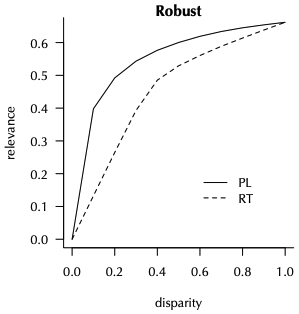
\includegraphics[width=\linewidth]{fig_diaz2020_fig3_robust.png}
\end{minipage}\hfill
\begin{minipage}{0.46\linewidth}
\centering
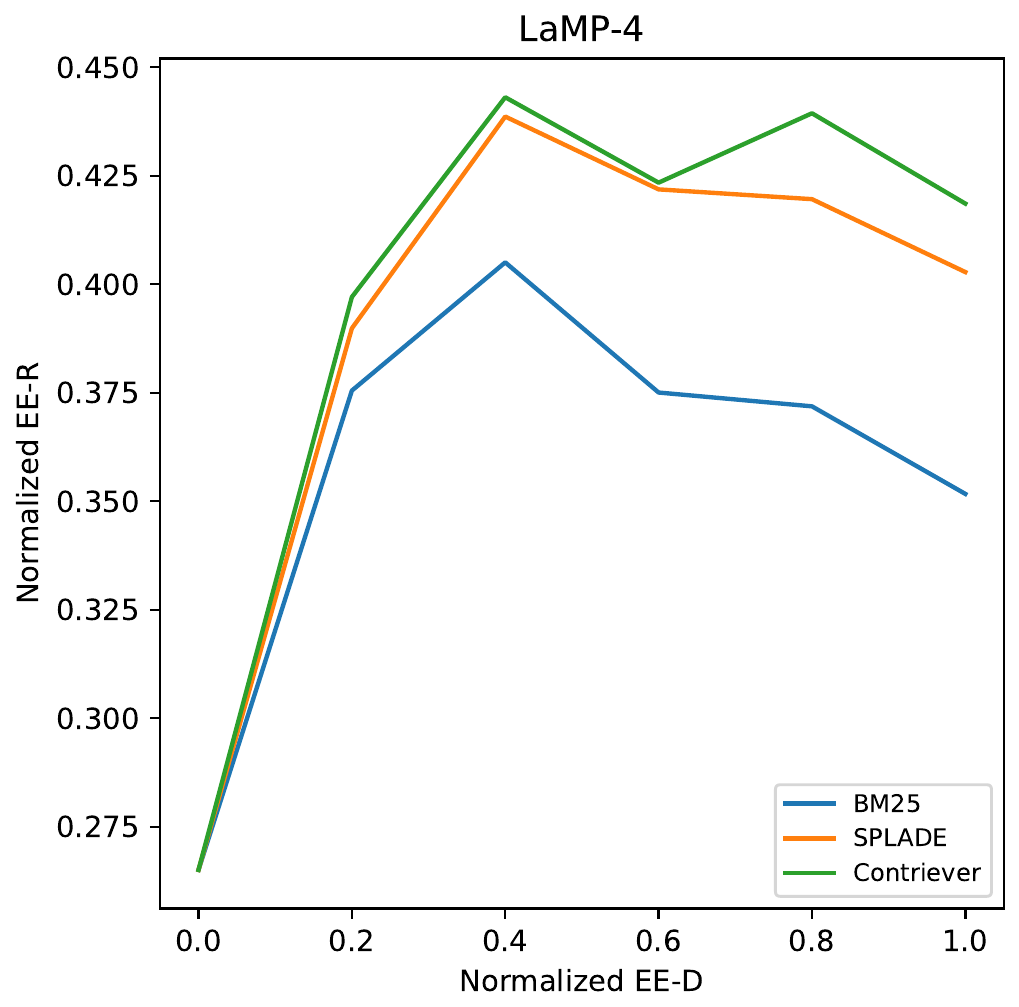
\includegraphics[width=\linewidth]{fig_source_4a_eeD_vs_eeR.png}
\end{minipage}
\caption{Textbook vs.\ observed fairness/quality trade-off. \emph{Left:} Diaz et
al.'s idealized disparity-vs-relevance curve for human users (Figure 3 of
\cite{diaz2020evaluating}), rising smoothly toward the fully-disparate optimum.
\emph{Right:} the source paper's own EE-D vs.\ EE-R curve for machine users
(Figure 4a of \cite{eunkim2025fairrag}, LaMP-4).}
\label{fig:diaz-vs-fairrag}
\end{figure}

\textbf{The source paper's own EE-D/EE-R relationship is non-monotonic.} The right
panel of Figure~\ref{fig:diaz-vs-fairrag} is the source paper's own Figure 4a:
unlike the textbook trade-off on the left, quality does not rise smoothly with
disparity. A dataset that doesn't behave like the typical case this framework
assumes raises a further concern about how representative LaMP is.

\section{Methodology Notes}
\label{sec:method}

We treat the original paper's open-sourced code as a direct reference throughout:
matching its library versions, reusing its utility-labeling technique
(Section~\ref{sec:threats}) and implementation details (prompt templates, scoring
functions) wherever our framework's structure allowed it directly, and otherwise
re-implementing to match its stated method as closely as we could. Two
compute-driven factors separate our reproduction from the source paper's own
numbers. First, Expected Utility needs one LLM call per sampled ranking; running
that at the paper's $N{=}100$ samples/query across 28 (task, generator, ranker)
cells and 4 PL settings was not feasible, so we use $N{=}10$ for EU throughout,
while EE-D --- which needs no generation --- stays at $N{=}100$ everywhere; this
asymmetry is not just a matter of compute cost, but numerically necessary
(Appendix~\ref{app:eed-bias}). Second,
our EU normalization ceiling (below) is built from fewer samples than the
paper's throughout --- only 3 random oracle permutations for gold\_ceiling, and
$N{=}10$ rather than $N{=}100$ for each model\_ceiling candidate --- so it is a
small, monotonically lower bound than a fuller-sample ceiling would give, which
can make our normalized EU somewhat higher than the paper's; see the per-cell
comparison against the paper's own numbers in Table~\ref{tab:baseline},
Appendix~\ref{app:baseline}.

Every EU$_{\text{norm}}$ value here uses the source paper's own per-query formula,
$\text{EU}_{\text{norm}}(q){=}\text{EU}(q)/\max(\text{gold\_ceiling}(q),
\text{model\_ceiling}(q))$ (Appendix C of \cite{eunkim2025fairrag}): raw utility
over the higher of a gold-ranked ceiling and a model ceiling --- the best output
any rerank method we ran produced for that query and (generator, ranker) pair,
whether PL, MMR, RandMMR, or deterministic. Appendix C of \cite{eunkim2025fairrag}
defines this bound for a fixed $\text{RAG}(R,G,k)$, and every method we run at a
given $(R,G,k)$ is a real empirical sample of it, falling back to $1.0$ when both
ceilings are zero.

\section{Results}
\label{sec:results}

\subsection{RQ1: Diversity as the mediating mechanism}
\label{sec:rq1}

RQ1 asks whether fairness's apparent lack of utility cost is really a diversity
effect in disguise. We first check the premise --- that PL's and MMR's dials actually
move measured diversity as intended --- before testing whether that diversity
predicts utility.

\begin{figure}[t]
\centering
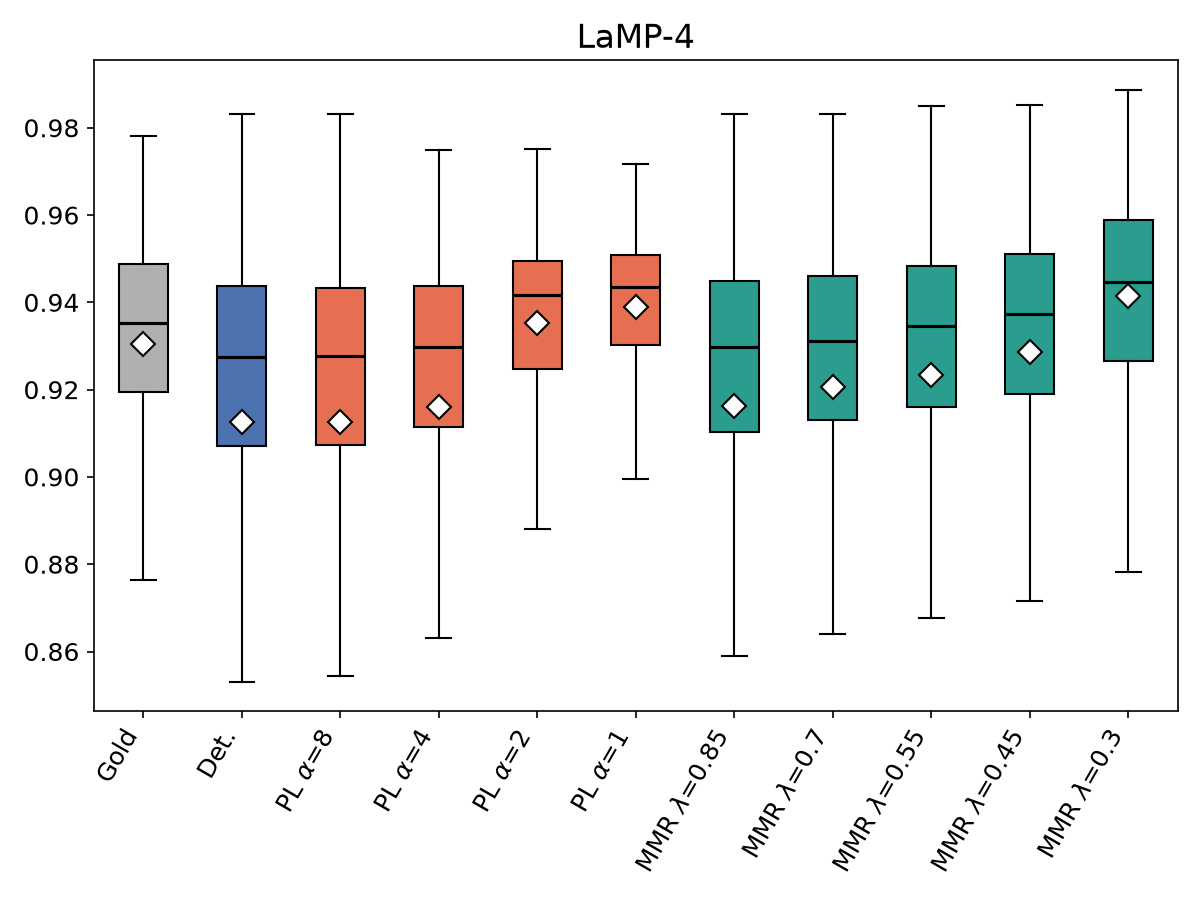
\includegraphics[width=\linewidth]{fig_diversity_lamp4_panel.png}
\caption{ILD-Jaccard diversity by rerank setting, LaMP-4. Diamond = mean, black
line = median. PL/MMR colors match Figure~\ref{fig:trend}'s legend.}
\label{fig:diversity}
\end{figure}

Figure~\ref{fig:diversity} shows LaMP-4 as a representative example: PL and MMR both
raise list diversity as their dial is relaxed ($\alpha{:}8{\to}1$,
$\lambda{:}0.85{\to}0.3$). The other six tasks show the same qualitative pattern.

The key test is whether this diversity increase predicts \emph{higher} utility.

\begin{figure}[t]
\centering
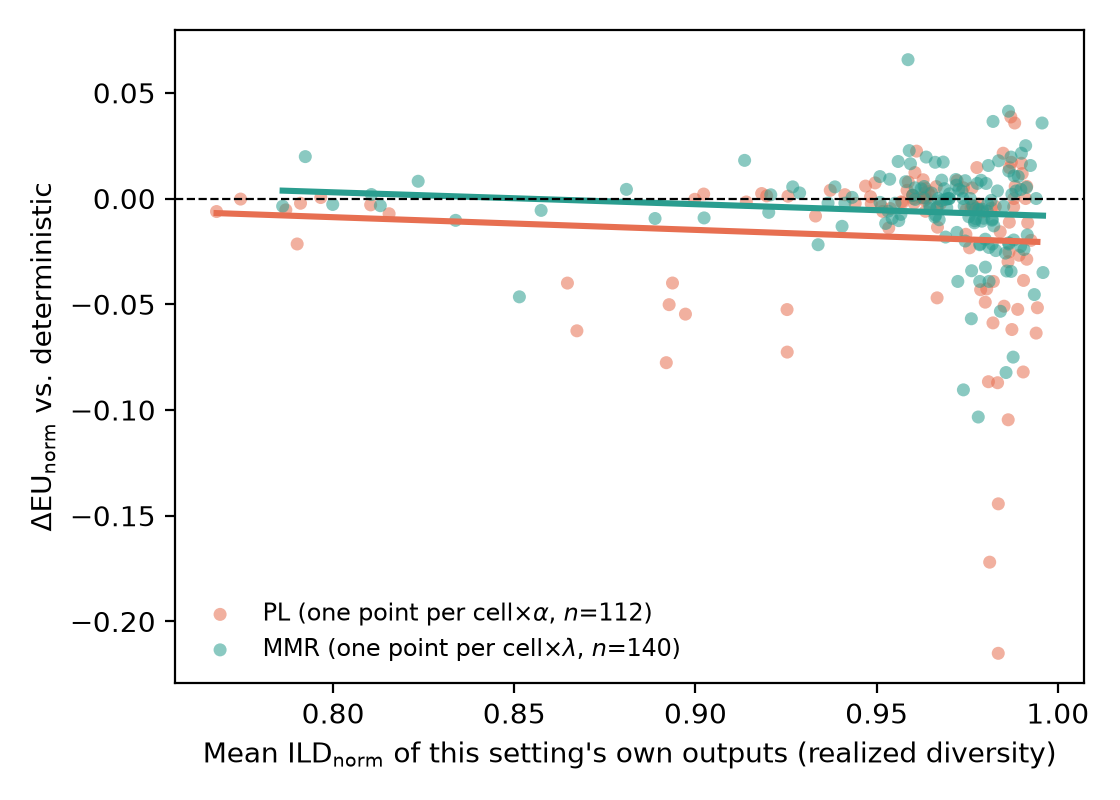
\includegraphics[width=\linewidth]{fig_diversity_trend_pooled.png}
\caption{$\Delta$EU$_{\text{norm}}$ vs.\ deterministic against realized diversity
(mean ILD$_{\text{norm}}$), pooled across all 28 cells; lines are least-squares
fits per method.}
\label{fig:trend}
\end{figure}

Figure~\ref{fig:trend} pools every (task, generator, ranker, setting) combination we
ran --- 112 PL points ($\alpha\in\{1,2,4,8\}$) and 140 MMR points
($\lambda\in\{0.3,0.45,0.55,0.7,0.85\}$), each plotting that setting's own realized
diversity against its utility gain over deterministic. Neither fitted trend rises:
PL's slope is negative (Spearman $\rho{=}{-}0.110$, $p{=}0.25$) and MMR's slightly
more so ($\rho{=}{-}0.164$, $p{=}0.053$) --- if anything, more diversity trends
toward \emph{less} utility gain, not more, though PL's downward pull is visibly
stronger than MMR's across the same range.

The same Figure~\ref{fig:trend} also shows that at matched diversity: PL and MMR
settings that realize almost identical diversity show MMR retaining more
utility than PL, however this is expected and doesn't carry a meaningful insight.

A third view compares each method's own best-case setting per cell, rather than
an average or a single fixed point: we wanted to see whether some MMR setting
decisively dominates PL, which would point to a specific level of diversity that
benefits utility. For each of the 28 cells, MMR's highest $\Delta$EU$_{\text{norm}}$
across its five $\lambda$ values against PL's highest across its four $\alpha$
values (Figure~\ref{fig:paired}). MMR's best beats PL's
best in 15 of 28 cells; the paired difference trends but falls just short of
significance. Only one task
is consistent across all four of its cells: LaMP-6, where MMR's best beats PL's
best in every (generator, ranker) combination. LaMP-7 leans the other way, MMR
winning only 1 of its 4 cells; the remaining five tasks split evenly, 2 cells
each way. If diversity-aware reranking helps any task specifically, LaMP-6 is
the only candidate --- though not by a statistically significant margin.

\begin{figure}[t]
\centering
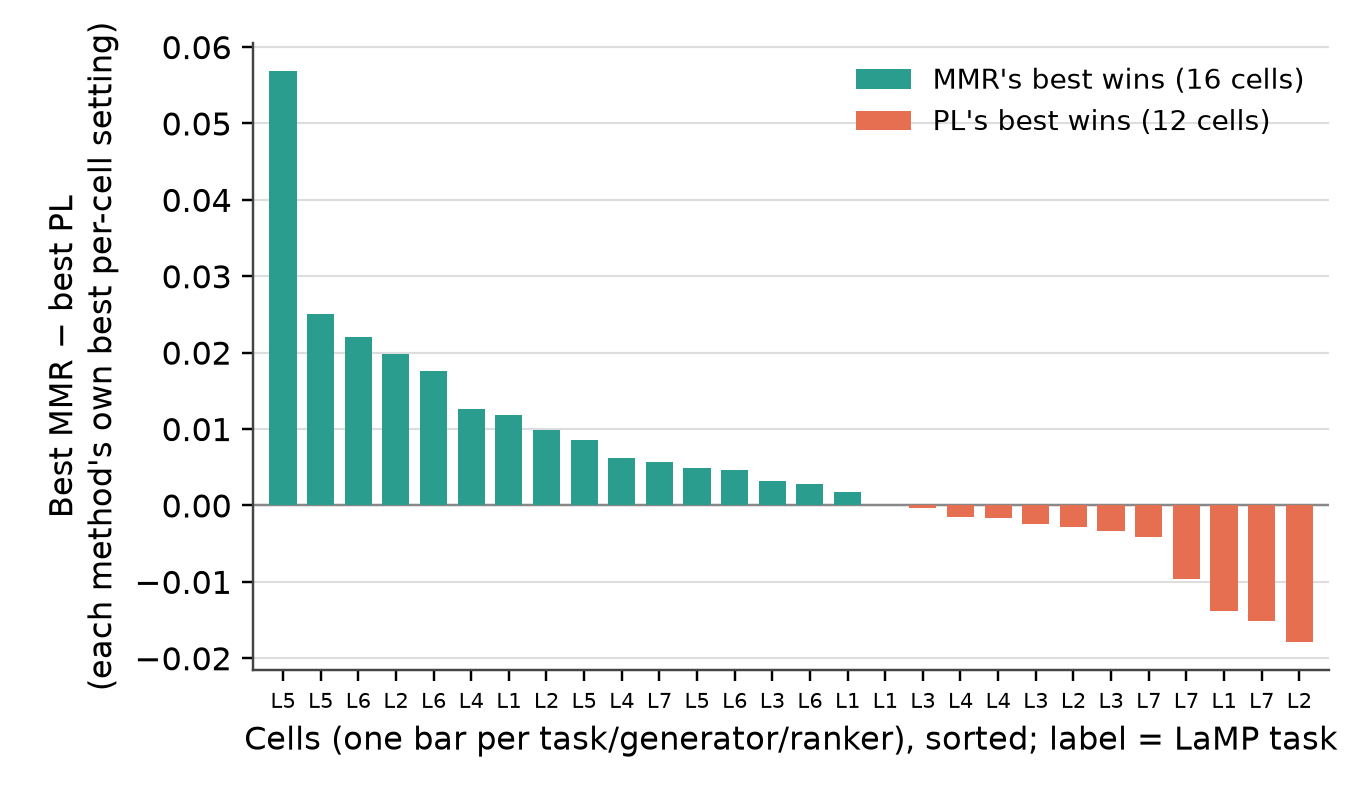
\includegraphics[width=\linewidth]{fig_best_mmr_vs_best_pl.png}
\caption{Best-case EU$_{\text{norm}}$, each method's own best-per-cell setting:
bar height is MMR's best minus PL's best. Per (task, generator, ranker) cell;
bars sorted, label = LaMP task.}
\label{fig:paired}
\end{figure}

Taken together, we could not verify the diversity-mediation hypothesis as
originally framed: neither method's utility rises with realized diversity, whether
pooled broadly (Table~\ref{tab:eu-full}, Appendix~\ref{app:eu-full}) or compared at specific matched points
(above).

\subsection{RQ2: RandMMR, a hybrid PL + randomized-MMR reranker}
\label{sec:rq2}

RQ1 found no evidence that diversity itself increases utility. However, we were
still curious whether combining PL's stochastic fairness mechanism with MMR's
diversification, which we call \textbf{RandMMR}, could synergize on
fairness rather than utility: layering diversification on top of randomization
might flatten the exposure distribution further than randomization alone,
lowering EE-D. RandMMR is not one fixed method but a small design space: the
PL temperature $\alpha$, how many of the top-$k$ ranks to randomize (just rank
1, or all $k$ of them), and the range $[\lambda_{\text{low}}, \lambda_{\text{high}}]$
that ranks $2..k$ draw their diversity weight from. Given a setting of these
parameters, RandMMR builds a ranking over the top-$k$ candidates as follows:

\begin{enumerate}[leftmargin=1.4em,itemsep=2pt]
  \item \textbf{Rank 1} is drawn via PL($\alpha$) in every variant: one
  Gumbel-max sample proportional to $\mathrm{score}(d,q)^\alpha$ over the initial
  ranking.
  \item \textbf{Ranks $2..k$}: at each rank $i$ being randomized, draw a fresh
  $\lambda \sim \mathrm{Unif}(\lambda_{\text{low}}, \lambda_{\text{high}})$, then
  pick the next document from the remaining candidates $\mathcal{C} \setminus S$
  (with $S$ the documents already selected at ranks $1..i{-}1$) either
  \emph{deterministically} --- the candidate maximizing MMR's score,
  Eq.~\eqref{eq:mmr} --- or \emph{stochastically}, drawing $d$ with probability
  proportional to its $\alpha$-sharpened relevance score times the diversity
  discount $\rho_\lambda(d) = 1 - (1-\lambda)\max_{d'\in S}\mathrm{sim}(d,d')$:
  \begin{equation}
  P_{\mathrm{randMMR}}(d \mid q, S) = \frac{\mathrm{score}(d,q)^\alpha\,\rho_\lambda(d)}
  {\displaystyle\sum_{d''\in\mathcal{C}\setminus S} \mathrm{score}(d'',q)^\alpha\,\rho_\lambda(d'')}.
  \label{eq:randmmr-stochastic}
  \end{equation}
  This is PL's own $P_{\mathrm{PL}}(d\mid q,S)$, Eq.~\eqref{eq:pl} --- the same
  $\alpha$-sharpened relevance term --- multiplicatively discounted by
  $\rho_\lambda$ rather than combined with it additively.\footnote{A different
  formulation is possible but untested by us: taking $\alpha$ over the
  already-discounted score rather than over relevance alone, $P(d\mid q,S) =
  \big(\mathrm{score}(d,q)\,\rho_\lambda(d)\big)^\alpha \big/
  \sum_{d''\in\mathcal{C}\setminus S} \big(\mathrm{score}(d'',q)\,\rho_\lambda(d'')\big)^\alpha$,
  so temperature sharpens relevance and diversity jointly instead of relevance
  alone.}
\end{enumerate}

The only setting we ran with a full utility comparison randomizes all $k$
ranks via the stochastic choice, $\alpha{=}4$, $\lambda\sim\mathrm{Unif}(0.8,1.0)$.
We evaluate it
against plain PL for every one of the 28 (task, generator, ranker) cells, with
EE-D computed at $N{=}100$ samples/query and EU at $N{=}10$
(Section~\ref{sec:method}). Each cell is matched to whichever PL
$\alpha \in \{1,2,4,8\}$ has EE-D closest to RandMMR's own, breaking ties toward
equal or \emph{higher} PL disparity so the comparison is not usually handed an
artificially fairer PL point to beat --- except within a 0.003 EE-D tolerance,
where the closest $\alpha$ is used regardless of direction. In every one of
the 28 cells, the matched $\alpha$ turns out to be 2.

\begin{table}[t]
\centering
\scriptsize
\setlength{\tabcolsep}{3pt}
\caption{RandMMR ($\alpha{=}4$, $\lambda\sim\mathrm{Unif}(0.8,1.0)$, all $k$
ranks randomized stochastically; see text) vs.\ matched plain PL
($\alpha{=}2$ in every row here), LaMP-1 and LaMP-4. EE-D and
EU are normalized per query to $[0,1]$ following the methodology in
Section~\ref{sec:method}. RandMMR's EE-D$_{\text{norm}}$ is lower (fairer) than
the matched PL's in every row shown; the other five LaMP tasks show a similar
pattern, given in full in Appendix~\ref{app:randmmr-full}
(Table~\ref{tab:hybrid-full}).}
\label{tab:hybrid}
\begin{tabular}{@{}ll rr r@{}}
\toprule
& & \multicolumn{2}{c}{EE-D$_{\text{norm}}$/EU$_{\text{norm}}$} & \\
\cmidrule(lr){3-4}
Task & Gen./Rank. & PL($\alpha{=}2$) & RandMMR & $\Delta$EU$_{\text{norm}}$ \\
\midrule
\multirow{4}{*}{LaMP-1} & Base/BM25    & 0.11/0.51 & 0.10/0.49 & $-$0.019 \\
 & Base/Contr.  & 0.10/0.56 & 0.09/0.51 & $-$0.048 \\
 & Small/BM25   & 0.10/0.40 & 0.08/0.39 & $-$0.008 \\
 & Small/Contr. & 0.09/0.39 & 0.08/0.41 & $+$0.020 \\
\cmidrule(lr){1-5}
\multirow{4}{*}{LaMP-4} & Base/BM25    & 0.18/0.25 & 0.17/0.25 & $+$0.003 \\
 & Base/Contr.  & 0.17/0.25 & 0.16/0.25 & $+$0.000 \\
 & Small/BM25   & 0.18/0.22 & 0.17/0.27 & $+$0.050$^{**}$ \\
 & Small/Contr. & 0.17/0.26 & 0.16/0.26 & $-$0.007 \\
\bottomrule
\end{tabular}
\end{table}

Table~\ref{tab:hybrid} shows the two tasks with a published baseline. RandMMR's
EU$_{\text{norm}}$ is higher than matched PL's in 4 of these 8 cells, one
significantly (Flan-T5-Small/BM25, LaMP-4, $+0.050$, $p{<}0.01$). Across the
remaining 20 cells (LaMP-2, 3, 5, 6, 7) it is higher in 8 of 20, one more
significantly (Flan-T5-Small/BM25, LaMP-2, $+0.108$, $p{<}0.05$). Overall,
RandMMR beats matched PL on utility in 12 of 28 cells (43\%), mean gain
$+0.003$: PL is ahead more often, but both statistically significant differences
favor RandMMR and none favor PL, both on the same (generator, ranker) pair,
Flan-T5-Small/BM25. We read this as a small hint of a real effect, not a
demonstrated win.

To see which toggle drives that fairness gain, Table~\ref{tab:toggle} adds the
first option from step 2 above (apply MMR, randomizing only rank 1), using EE-D
alone since it needs no generation, for one representative cell (LaMP-1,
Flan-T5-Base/BM25, $N{=}100$); the same pattern holds across the other
settings we checked.

\begin{table}[t]
\centering
\scriptsize
\setlength{\tabcolsep}{4pt}
\caption{``Ranks randomized using PL'' is how many of the top-$k$ picks are
drawn stochastically via PL rather than chosen deterministically by MMR
score.}
\label{tab:toggle}
\begin{tabular}{@{}ll cc r@{}}
\toprule
Setting & Ranks randomized using PL & $\alpha$ & $\lambda$ & EE-D \\
\midrule
Plain PL & all $k$ & 1 & --- & 0.073 \\
Plain PL & all $k$ & 2 & --- & 0.115 \\
Plain PL & all $k$ & 4 & --- & 0.682 \\
Plain PL & all $k$ & 8 & --- & 0.965 \\
\cmidrule(lr){1-5}
RandMMR (Table~\ref{tab:hybrid}) & all $k$ & 4 & $U(0.8,1.0)$ & 0.099 \\
RandMMR & all $k$ & 4 & $0.9$ (fixed) & 0.099 \\
RandMMR & all $k$ & 8 & $U(0.8,1.0)$ & 0.223 \\
RandMMR & all $k$ & 8 & $0.9$ (fixed) & 0.223 \\
RandMMR & rank 1 only & 4 & $U(0.8,1.0)$ & 0.804 \\
RandMMR & rank 1 only & 4 & $0.9$ (fixed) & 0.810 \\
RandMMR & rank 1 only & 8 & $U(0.8,1.0)$ & 0.838 \\
RandMMR & rank 1 only & 8 & $0.9$ (fixed) & 0.843 \\
\bottomrule
\end{tabular}
\end{table}

Randomizing all $k$ ranks is far more effective than randomizing only rank 1,
regardless of $\alpha$: at $\alpha{=}4$ it takes the raw PL draw from 0.682
down to 0.099, and at $\alpha{=}8$, from 0.965 down to 0.223 --- fixed vs.\
ranged $\lambda$ makes no real difference either way. Randomizing only rank 1
is far weaker: 0.80--0.81 at $\alpha{=}4$ and 0.84 at $\alpha{=}8$, both still
close to plain PL($\alpha{=}8$)'s own 0.965. This follows from the mechanism:
under rank-1-only randomization, ranks $2..k$ are chosen by deterministic MMR
argmax regardless of $\alpha$, so they dominate EE-D, with $\alpha$ only
shifting how peaked rank 1 itself is. Fixed vs.\ resampled $\lambda$ again
barely matters (differences $\leq$0.006 throughout): for both mechanisms, the
gain comes from how many ranks are randomized, not from how $\lambda$ is
chosen within an otherwise-deterministic tail. We read this as a modestly
optimistic sign: adding diversity-aware structure to PL need not cost more
than plain PL already costs at that $\alpha$, and randomizing the full list
can lower disparity substantially even where plain PL alone is nearly fully
deterministic --- worth testing on a dataset where diversity is known to help
utility, which RQ1 suggests LaMP may not be.

\FloatBarrier
\section{Conclusions and Future Work}
\label{sec:conclusion}

We set out to test whether the source paper's finding --- that fairness-aware
stochastic reranking does not cost RAG generation utility --- is explained by an
increase in retrieved-item diversity. We found no evidence that it is, as seen
in Section~\ref{sec:rq1}. Along the way we found reasons to believe that the
utility retention with fairness interventions is explained by an unusual and
noisy dataset (Section~\ref{sec:threats}). RandMMR, our proposed hybrid of
PL's fairness draw and MMR's diversification, does not clearly beat plain PL
on utility either, but is more consistently fairer (Section~\ref{sec:rq2}) ---
a promising direction.

Despite not confirming our initial hypothesis, we see real potential in a few
directions a proper follow-up should pursue:

\begin{enumerate}[leftmargin=1.1em,itemsep=3pt]
  \item \textbf{Scale and realism.} Nearly every number in this paper comes
  from a setup chosen for what we could afford computationally, and as this is a course project, compromises were made:
  small sample counts, generators far below production scale, a ground
  truth that depends on those same small generators' own judgments, and a
  ROUGE-L-based utility signal standing in for a more precise but far costlier
  LLM-as-judge evaluation on the four generation tasks --- including the
  generator-scale gap already noted in Section~\ref{sec:threats}. A repeat at
  industry scale, with bigger sample counts, a
  dataset whose relevance labels do not depend on a single generator's own
  utility delta, and utility scored closer to human judgment than ROUGE-L
  allows, would show how much of RQ1--RQ2 survives outside this regime.
  \item \textbf{Task-specific RAG fairness-diversity balancing.} An interesting course of research in our opinion would be to study how much diversity is beneficial depending on the specific task or query (also outside of LaMP dataset) and how it can be balanced with fairness constraints in an optimal way.
  \item \textbf{Other reranking designs, and validating RandMMR properly.} We have
  only measured utility for one point in RandMMR's design space (all $k$ ranks
  randomized); the two narrower, EE-D-only variants above are promising but
  untested for utility, and neither is the only way to combine PL and MMR.
  Comparing more points in this space, and against diversity/fairness methods
  outside the PL/MMR family entirely (e.g.\ explicit sub-topic-coverage
  diversification), could be an interesting research direction and may possibly
  yield another diversity-fairness balancing algorithm.
\end{enumerate}

\newpage
{\footnotesize
\begin{thebibliography}{99}

\bibitem{eunkim2025fairrag}
T.\ Eun Kim and F.\ Diaz.
\newblock Towards Fair RAG: On the Impact of Fair Ranking in Retrieval-Augmented
Generation.
\newblock \emph{ICTIR}, 2025. arXiv:2409.11598.

\bibitem{castillo2018fairness}
C.\ Castillo.
\newblock Fairness and Transparency in Ranking.
\newblock \emph{ACM SIGIR Forum}, 52(2), 2018.

\bibitem{diaz2020evaluating}
F.\ Diaz, B.\ Mitra, M.\ D.\ Ekstrand, A.\ J.\ Biega, and B.\ Carterette.
\newblock Evaluating Stochastic Rankings with Expected Exposure.
\newblock \emph{CIKM}, 2020.

\bibitem{salemi2023lamp}
A.\ Salemi, S.\ Mysore, M.\ Bendersky, and H.\ Zamani.
\newblock LaMP: When Large Language Models Meet Personalization.
\newblock arXiv:2304.11406, 2023.

\bibitem{chung2024scaling}
H.\ W.\ Chung et al.
\newblock Scaling Instruction-Finetuned Language Models.
\newblock \emph{JMLR}, 25, 2024.

\bibitem{carbonell1998use}
J.\ Carbonell and J.\ Goldstein.
\newblock The Use of MMR, Diversity-Based Reranking for Reordering Documents and
Producing Summaries.
\newblock \emph{SIGIR}, 1998.

\bibitem{smyth2001similarity}
B.\ Smyth and P.\ McClave.
\newblock Similarity vs.\ Diversity.
\newblock \emph{ICCBR}, 2001.

\bibitem{plackett1975analysis}
R.\ L.\ Plackett.
\newblock The Analysis of Permutations.
\newblock \emph{Journal of the Royal Statistical Society: Series C}, 24(2), 1975.

\bibitem{luce1959individual}
R.\ D.\ Luce.
\newblock \emph{Individual Choice Behavior: A Theoretical Analysis}.
\newblock Wiley, 1959.

\end{thebibliography}
}

\clearpage
\appendix
\section{LaMP Corpus Statistics}
\label{app:corpus}

Table~\ref{tab:corpus} gives the per-task, per-generator candidate-pool sizes and
useful-document rates summarized in Section~\ref{sec:threats}.

\begin{table*}[t]
\centering
\scriptsize
\caption{LaMP candidate-pool size and useful- (i.e.\ relevant-) document rate, per task and generator (from each task's relevance-mapping file).}
\label{tab:corpus}
\begin{tabular}{@{}lrrrrrrrrrrrrrr@{}}
\toprule
& \multicolumn{2}{c}{LaMP-1} & \multicolumn{2}{c}{LaMP-2} & \multicolumn{2}{c}{LaMP-3} & \multicolumn{2}{c}{LaMP-4} & \multicolumn{2}{c}{LaMP-5} & \multicolumn{2}{c}{LaMP-6} & \multicolumn{2}{c}{LaMP-7} \\
Generator & cand. & \%use & cand. & \%use & cand. & \%use & cand. & \%use & cand. & \%use & cand. & \%use & cand. & \%use \\
\midrule
Flan-T5-Small & 123.5 & 9.5 & 52.8 & 22.5 & 189.8 & 34.3 & 192.2 & 27.1 & 106.1 & 24.8 & 86.0 & 35.9 & 19.4 & 45.5 \\
Flan-T5-Base  & 102.9 & 22.5 & 45.6 & 29.9 & 185.3 & 41.2 & 187.0 & 31.6 & 105.6 & 25.7 & 86.2 & 38.6 & 21.7 & 33.0 \\
\bottomrule
\end{tabular}
\end{table*}

\section{Sample-Size Asymmetry Between EE-D and EU}
\label{app:eed-bias}

Section~\ref{sec:method} holds EE-D at $N{=}100$ samples/query while using only
$N{=}10$ for EU. This is not purely a compute-cost choice: the two metrics are
estimated from $N$ sampled rankings in structurally different ways, and only one
of them is biased by a small $N$.

EE-D is a Monte Carlo estimate of a squared $L_2$ norm,
$\widehat{\text{EE-D}} = \lVert \hat\epsilon \rVert_2^2$, where
$\hat\epsilon_d = \frac{1}{N}\sum_{i=1}^N \mathrm{MU}(\bar\pi^{(i)}_d)$ is the
sample-mean exposure of item $d$ across the $N$ sampled rankings
(Section~\ref{sec:related}). Since $\mathrm{MU}(\cdot) \in \{0,1\}$,
$\hat\epsilon_d$ is a sample proportion with
$\mathrm{Var}(\hat\epsilon_d) = \epsilon_d(1{-}\epsilon_d)/N$, so
\begin{align*}
\mathbb{E}\big[\widehat{\text{EE-D}}\big] &= \sum_d \mathbb{E}[\hat\epsilon_d^2]
= \sum_d \big(\epsilon_d^2 + \mathrm{Var}(\hat\epsilon_d)\big) \\
&= \lVert \epsilon \rVert_2^2 + \frac{1}{N}\sum_d \epsilon_d(1{-}\epsilon_d).
\end{align*}
The squared-norm estimator is therefore biased \emph{upward} by a term that
shrinks monotonically as $N$ grows: a small $N$ systematically overstates
disparity, and only a large $N$ brings the estimate close to the true
(infinite-sample) EE-D. $N{=}100$, the source paper's own choice, is large
enough that this bias is negligible; since EE-D needs no generation, we can
afford to match it everywhere.

EU has no equivalent structural bias. It is a plain sample mean of per-ranking
task scores, $\widehat{\text{EU}}(q) = \frac{1}{N}\sum_{i=1}^N
\text{score}(\pi^{(i)}, q)$, which is unbiased at any $N$ --- a smaller $N$ adds
variance (noisier per-query estimates) but no systematic directional error. That
asymmetry is why we accept $N{=}10$ for EU, where each sample costs one LLM call,
while holding EE-D at the paper's own $N{=}100$.

\section{Deterministic-Baseline EU Detail}
\label{app:baseline}

Table~\ref{tab:baseline} compares our reproduction against the source paper's own
Table 2 two ways at once: a single deterministic-baseline EU$_{\text{norm}}$ value
per (retriever, generator) cell (Section~\ref{sec:method} for the formula) and,
following the source paper's own Table 2 exactly, the mean utility gain of
PL-sampled rankings over that baseline, pooled across all four PL $\alpha$ values
and binned into the same five EE-D disparity intervals the paper uses. Each row is
one (retriever, generator) cell for one of the two tasks the paper publishes this
comparison for; every cell shows Ours/Paper together.

On LaMP-1, a binary decision (accuracy over two candidate labels), the divergence is
generator-driven: Flan-T5-Base's baseline stays within 1--2\% of the paper, while
Flan-T5-Small diverges 46--51\% \emph{above} it. We traced this to a
content-invariant failure mode specific to Small on this task (Section~\ref{sec:method}):
it predicts the same label regardless of which document is retrieved, so its accuracy
reduces to how often that fixed label happens to be correct rather than reflecting
ranking quality --- and because gold\_ceiling is computed from that same
content-invariant behavior, it tracks the deterministic baseline almost exactly for
whichever queries the fixed label happens to get right, making the normalized value
unstable rather than a meaningful closeness-to-optimal measure. This makes Small's
LaMP-1 numbers intrinsically noisy at this sample size, independent of anything about
the reranker.

On LaMP-4, all four cells diverge in the same direction, above the paper, and now
much more uniformly than LaMP-1: 27--30\% for Flan-T5-Base, 28--37\% for
Flan-T5-Small --- the two generators sit far closer together here than on LaMP-1,
and Flan-T5-Small/BM25 no longer stands out as an outlier (37\%, in line with the
other three cells). This is a normalization-ceiling gap, not a generation-quality
one: our model\_ceiling is the best utility any rerank method we ran ever observed
for a query --- PL at any $\alpha$, MMR at any $\lambda$, or deterministic ---
taken together with gold\_ceiling above, rather than an exhaustive search over the
many permutations and subsets of a query's useful documents that could occupy the
$k{=}5$ slots. That search was not computationally feasible at this project's scale
(Section~\ref{sec:threats}), so our ceiling likely still sits below the paper's own
whenever a query has more useful documents than fit in $k{=}5$; since EU is raw
utility divided by this ceiling, a lower ceiling mechanically inflates our
normalized value for the same underlying generation quality.

The interval columns add a view the single baseline number cannot: how utility gain
over baseline changes as fairness (lower EE-D) increases. Six of the eight cells are
negative and significant at the lowest disparity interval ($[0,0.2)$, where the
fairness intervention is most aggressive), matching the paper's own pattern there
exactly (same six cells); two of those (both on LaMP-4, Contriever) stay significant
through the second interval before recovering toward zero. Flan-T5-Small/BM25 on
LaMP-4 shows a different pattern instead, significant again at $[.6,.8)$
($n{=}80$) rather than at the second interval --- still far from the
four-of-five-interval divergence this cell showed under an earlier, PL-only
normalization ceiling, but no longer the single clean matching interval it showed
under a smaller EE-D sample. Flan-T5-Small's two LaMP-1 cells remain the noisiest:
Contriever+Small shows no significant interval in either direction, and
BM25+Small's nominal significance at $[.2,.4)$ rests on only 2 queries in that bin
--- not a meaningful result, and consistent with the small-sample noise already
discussed above for this cell.

The \emph{relative} pattern the paper's own Table 2 shows --- Flan-T5-Base above
Flan-T5-Small, BM25 above Contriever on LaMP-1, Contriever above BM25 on LaMP-4 ---
now survives almost entirely. The single exception is LaMP-4/BM25, where Small edges
narrowly ahead of Base (0.30 vs.\ 0.29); every other comparison, including both
retriever orderings for Flan-T5-Small (BM25 above Contriever on LaMP-1, Contriever
above BM25 on LaMP-4), now matches the paper. Under the previous PL-only ceiling,
Small violated both of those retriever orderings; broadening the ceiling resolved
them along with the interval-column outlier noted above.

\begin{table*}[t]
\centering
\scriptsize
\caption{Our reproduction vs.\ the source paper's own Table 2 (see text),
Ours/Paper in every cell. $^*p{<}0.05$ (ours: Welch's $t$-test vs.\ pooled
baseline; paper: unpaired Student's, per their Table 2 caption). $^\dagger$this
interval has only 2 queries for this cell; not a meaningful result despite
$p{<}0.05$.}
\label{tab:baseline}
\begin{tabular}{@{}llcccccc@{}}
\toprule
Task & Retriever+Gen. & Baseline & [.0,.2) & [.2,.4) & [.4,.6) & [.6,.8) & [.8,1.0] \\
\midrule
LaMP-1 & BM25+Base   & 0.68/0.67 & $-$0.20$^{*}$/$-$0.20$^{*}$ & $-$0.01/$-$0.04 & $-$0.08/$-$0.08 & $-$0.04/$-$0.05 & $-$0.02/$-$0.02 \\
LaMP-1 & Contr.+Base & 0.64/0.64 & $-$0.12$^{*}$/$-$0.16$^{*}$ & $+$0.07/$+$0.05 & $-$0.04/$-$0.06 & $+$0.05/$+$0.03 & $+$0.00/$+$0.00 \\
LaMP-1 & BM25+Small  & 0.45/0.31 & $-$0.06/$-$0.12 & $-$0.43$^{*\dagger}$/$-$0.13 & $+$0.08/$-$0.18 & $+$0.07/$-$0.02 & $-$0.03/$-$0.15 \\
LaMP-1 & Contr.+Small& 0.43/0.29 & $-$0.04/$-$0.08 & $-$0.43/$-$0.29 & $-$0.15/$-$0.06 & $+$0.15/$+$0.03 & $-$0.02/$-$0.14 \\
\midrule
LaMP-4 & BM25+Base   & 0.29/0.22 & $-$0.08$^{*}$/$-$0.06$^{*}$ & $-$0.01/$+$0.00 & $+$0.03/$+$0.03 & $+$0.00/$+$0.01 & $+$0.00/$+$0.02 \\
LaMP-4 & Contr.+Base & 0.34/0.27 & $-$0.12$^{*}$/$-$0.10$^{*}$ & $-$0.03$^{*}$/$-$0.02 & $+$0.02/$+$0.01 & $-$0.01/$+$0.00 & $+$0.00/$+$0.01 \\
LaMP-4 & BM25+Small  & 0.30/0.22 & $-$0.11$^{*}$/$-$0.06$^{*}$ & $-$0.02/$+$0.00 & $+$0.00/$+$0.02 & $-$0.06$^{*}$/$+$0.01 & $-$0.00/$+$0.00 \\
LaMP-4 & Contr.+Small& 0.33/0.25 & $-$0.09$^{*}$/$-$0.09$^{*}$ & $-$0.03$^{*}$/$-$0.02$^{*}$ & $-$0.00/$+$0.00 & $+$0.02/$+$0.01 & $+$0.00/$+$0.00 \\
\bottomrule
\end{tabular}
\end{table*}

\section{Full EU$_{\text{norm}}$ by Setting}
\label{app:eu-full}

Table~\ref{tab:eu-full} gives the per-cell EU$_{\text{norm}}$ (Section~\ref{sec:method})
underlying Section~\ref{sec:rq1}'s pooled and matched-point comparisons: the
deterministic baseline, PL at each $\alpha \in \{1,2,4,8\}$, and MMR at each
$\lambda \in \{0.3,0.45,0.55,0.7,0.85\}$ we report elsewhere in the paper (MMR was
also run at $\lambda{=}0.15$; we omit that column here since it falls outside the
$\lambda$ range used in the rest of the paper, Section~\ref{sec:data}).

\begin{table*}[t]
\centering
\scriptsize
\setlength{\tabcolsep}{3.2pt}
\caption{EU$_{\text{norm}}$ by setting, all 28 (task, generator, ranker) cells.
Det.\ = deterministic baseline; PL$_\alpha$ = Plackett-Luce at temperature
$\alpha$; M$_\lambda$ = MMR at diversity weight $\lambda$.}
\label{tab:eu-full}
\begin{tabular}{@{}lll rrrrr rrrrr@{}}
\toprule
& & & & \multicolumn{4}{c}{PL} & \multicolumn{5}{c}{MMR} \\
\cmidrule(lr){5-8}\cmidrule(lr){9-13}
Task & Gen. & Rank. & Det. & $\alpha{=}1$ & $\alpha{=}2$ & $\alpha{=}4$ & $\alpha{=}8$
& $\lambda{=}.3$ & $\lambda{=}.45$ & $\lambda{=}.55$ & $\lambda{=}.7$ & $\lambda{=}.85$ \\
\midrule
LaMP-1 & Base & BM25 & 0.68 & 0.47 & 0.51 & 0.63 & 0.67 & 0.65 & 0.66 & 0.66 & 0.67 & 0.68 \\
 & Base & Contr. & 0.64 & 0.50 & 0.56 & 0.66 & 0.65 & 0.62 & 0.63 & 0.65 & 0.65 & 0.64 \\
 & Small & BM25 & 0.45 & 0.39 & 0.40 & 0.45 & 0.45 & 0.43 & 0.41 & 0.41 & 0.41 & 0.45 \\
 & Small & Contr. & 0.43 & 0.39 & 0.39 & 0.44 & 0.43 & 0.45 & 0.43 & 0.43 & 0.43 & 0.45 \\
LaMP-2 & Base & BM25 & 0.30 & 0.34 & 0.32 & 0.31 & 0.30 & 0.32 & 0.31 & 0.29 & 0.31 & 0.30 \\
 & Base & Contr. & 0.31 & 0.31 & 0.32 & 0.35 & 0.32 & 0.34 & 0.33 & 0.33 & 0.31 & 0.32 \\
 & Small & BM25 & 0.33 & 0.35 & 0.35 & 0.33 & 0.33 & 0.28 & 0.37 & 0.35 & 0.23 & 0.33 \\
 & Small & Contr. & 0.38 & 0.36 & 0.38 & 0.38 & 0.38 & 0.34 & 0.39 & 0.38 & 0.30 & 0.39 \\
LaMP-3 & Base & BM25 & 0.92 & 0.93 & 0.93 & 0.92 & 0.92 & 0.92 & 0.92 & 0.92 & 0.93 & 0.92 \\
 & Base & Contr. & 0.93 & 0.92 & 0.92 & 0.93 & 0.93 & 0.93 & 0.93 & 0.93 & 0.93 & 0.93 \\
 & Small & BM25 & 0.91 & 0.88 & 0.89 & 0.90 & 0.91 & 0.88 & 0.89 & 0.90 & 0.89 & 0.91 \\
 & Small & Contr. & 0.90 & 0.89 & 0.89 & 0.90 & 0.90 & 0.87 & 0.89 & 0.90 & 0.89 & 0.90 \\
LaMP-4 & Base & BM25 & 0.29 & 0.24 & 0.25 & 0.29 & 0.29 & 0.29 & 0.30 & 0.29 & 0.30 & 0.29 \\
 & Base & Contr. & 0.34 & 0.23 & 0.25 & 0.34 & 0.34 & 0.34 & 0.33 & 0.34 & 0.34 & 0.34 \\
 & Small & BM25 & 0.30 & 0.27 & 0.28 & 0.30 & 0.30 & 0.21 & 0.31 & 0.31 & 0.21 & 0.30 \\
 & Small & Contr. & 0.33 & 0.24 & 0.26 & 0.32 & 0.33 & 0.30 & 0.32 & 0.32 & 0.29 & 0.33 \\
LaMP-5 & Base & BM25 & 0.53 & 0.52 & 0.53 & 0.54 & 0.54 & 0.54 & 0.54 & 0.55 & 0.55 & 0.54 \\
 & Base & Contr. & 0.55 & 0.52 & 0.53 & 0.55 & 0.55 & 0.54 & 0.55 & 0.55 & 0.56 & 0.56 \\
 & Small & BM25 & 0.46 & 0.41 & 0.42 & 0.47 & 0.46 & 0.50 & 0.47 & 0.47 & 0.52 & 0.46 \\
 & Small & Contr. & 0.46 & 0.40 & 0.41 & 0.46 & 0.46 & 0.46 & 0.45 & 0.46 & 0.49 & 0.45 \\
LaMP-6 & Base & BM25 & 0.47 & 0.40 & 0.41 & 0.45 & 0.47 & 0.46 & 0.46 & 0.47 & 0.47 & 0.47 \\
 & Base & Contr. & 0.44 & 0.39 & 0.40 & 0.44 & 0.44 & 0.42 & 0.44 & 0.45 & 0.43 & 0.44 \\
 & Small & BM25 & 0.44 & 0.37 & 0.39 & 0.43 & 0.44 & 0.41 & 0.42 & 0.43 & 0.46 & 0.44 \\
 & Small & Contr. & 0.42 & 0.37 & 0.38 & 0.42 & 0.42 & 0.37 & 0.44 & 0.44 & 0.38 & 0.43 \\
LaMP-7 & Base & BM25 & 0.67 & 0.66 & 0.66 & 0.66 & 0.67 & 0.64 & 0.65 & 0.66 & 0.67 & 0.66 \\
 & Base & Contr. & 0.65 & 0.65 & 0.65 & 0.65 & 0.65 & 0.65 & 0.64 & 0.64 & 0.64 & 0.64 \\
 & Small & BM25 & 0.54 & 0.53 & 0.53 & 0.54 & 0.54 & 0.51 & 0.51 & 0.52 & 0.53 & 0.53 \\
 & Small & Contr. & 0.53 & 0.53 & 0.52 & 0.53 & 0.53 & 0.48 & 0.51 & 0.52 & 0.51 & 0.52 \\
\bottomrule
\end{tabular}
\end{table*}

\section{Full RandMMR vs.\ Plain-PL Comparison}
\label{app:randmmr-full}

Table~\ref{tab:hybrid-full} gives the complete per-cell detail behind
Section~\ref{sec:rq2}'s 12-of-28 tally (Table~\ref{tab:hybrid} in the main text shows
only the two tasks with a published baseline). Columns are as in
Table~\ref{tab:hybrid}: PL $\alpha$ is the plain-PL condition matched to RandMMR's own
EE-D for that cell (uniformly $\alpha{=}2$ here), and
$\Delta$EU is RandMMR's EU$_{\text{norm}}$ minus the matched PL's. EE-D is computed
at $N{=}100$ samples/query, EU at $N{=}10$ (Section~\ref{sec:method}), for every
cell in the table.

\begin{table*}[t]
\centering
\scriptsize
\caption{RandMMR ($\alpha{=}4$, $\lambda\sim\mathrm{Unif}(0.8,1.0)$, all $k$
ranks randomized stochastically; see text) vs.\ matched plain PL (PL $\alpha$
column, matched per cell as described in Section~\ref{sec:rq2}), all
$7\times4{=}28$ cells, EE-D at $N{=}100$, EU at $N{=}10$. $^{*}p{<}0.05$,
$^{**}p{<}0.01$ (Welch's $t$-test vs.\ matched PL).}
\label{tab:hybrid-full}
\begin{tabular}{@{}lllrllr@{}}
\toprule
Task & Generator & Ranker & PL $\alpha$ & PL EE-D$_{\text{norm}}$/EU$_{\text{norm}}$ & RandMMR EE-D$_{\text{norm}}$/EU$_{\text{norm}}$ & $\Delta$EU$_{\text{norm}}$ \\
\midrule
\multirow{4}{*}{LaMP-1} & T5-Base & BM25 & 2 & 0.11/0.51 & 0.10/0.49 & $-0.019$ \\
 & T5-Base & Contriever & 2 & 0.10/0.56 & 0.09/0.51 & $-0.048$ \\
 & T5-Small & BM25 & 2 & 0.10/0.40 & 0.08/0.39 & $-0.008$ \\
 & T5-Small & Contriever & 2 & 0.09/0.39 & 0.08/0.41 & $+0.020$ \\
\cmidrule(lr){1-7}
\multirow{4}{*}{LaMP-2} & T5-Base & BM25 & 2 & 0.32/0.32 & 0.30/0.31 & $-0.008$ \\
 & T5-Base & Contriever & 2 & 0.32/0.32 & 0.30/0.31 & $-0.006$ \\
 & T5-Small & BM25 & 2 & 0.29/0.24 & 0.28/0.35 & $+0.108^{*}$ \\
 & T5-Small & Contriever & 2 & 0.29/0.38 & 0.28/0.37 & $-0.011$ \\
\cmidrule(lr){1-7}
\multirow{4}{*}{LaMP-3} & T5-Base & BM25 & 2 & 0.07/0.93 & 0.06/0.93 & $-0.001$ \\
 & T5-Base & Contriever & 2 & 0.06/0.92 & 0.05/0.92 & $-0.001$ \\
 & T5-Small & BM25 & 2 & 0.06/0.87 & 0.05/0.89 & $+0.016$ \\
 & T5-Small & Contriever & 2 & 0.06/0.89 & 0.05/0.89 & $-0.000$ \\
\cmidrule(lr){1-7}
\multirow{4}{*}{LaMP-4} & T5-Base & BM25 & 2 & 0.18/0.25 & 0.17/0.25 & $+0.003$ \\
 & T5-Base & Contriever & 2 & 0.17/0.25 & 0.16/0.25 & $+0.000$ \\
 & T5-Small & BM25 & 2 & 0.18/0.22 & 0.17/0.27 & $+0.050^{**}$ \\
 & T5-Small & Contriever & 2 & 0.17/0.26 & 0.16/0.26 & $-0.007$ \\
\cmidrule(lr){1-7}
\multirow{4}{*}{LaMP-5} & T5-Base & BM25 & 2 & 0.10/0.53 & 0.09/0.53 & $+0.002$ \\
 & T5-Base & Contriever & 2 & 0.11/0.53 & 0.09/0.53 & $+0.002$ \\
 & T5-Small & BM25 & 2 & 0.10/0.42 & 0.09/0.41 & $-0.007$ \\
 & T5-Small & Contriever & 2 & 0.11/0.41 & 0.09/0.41 & $-0.006$ \\
\cmidrule(lr){1-7}
\multirow{4}{*}{LaMP-6} & T5-Base & BM25 & 2 & 0.16/0.41 & 0.15/0.41 & $+0.001$ \\
 & T5-Base & Contriever & 2 & 0.16/0.40 & 0.14/0.40 & $-0.001$ \\
 & T5-Small & BM25 & 2 & 0.16/0.39 & 0.15/0.39 & $-0.001$ \\
 & T5-Small & Contriever & 2 & 0.16/0.38 & 0.14/0.38 & $-0.002$ \\
\cmidrule(lr){1-7}
\multirow{4}{*}{LaMP-7} & T5-Base & BM25 & 2 & 0.47/0.66 & 0.47/0.65 & $-0.007$ \\
 & T5-Base & Contriever & 2 & 0.44/0.65 & 0.42/0.65 & $+0.004$ \\
 & T5-Small & BM25 & 2 & 0.50/0.53 & 0.50/0.54 & $+0.009$ \\
 & T5-Small & Contriever & 2 & 0.48/0.52 & 0.47/0.53 & $+0.001$ \\
\bottomrule
\end{tabular}
\end{table*}

\end{document}
